\scanpage{22}
\uline{Correction} \quad If $G$ affine monoid of finite type over field $k$, we have a multiplicative closed immersion $G\mathbin{-}\mathbb M_{\unsure{n,k|n\,k}}$ (not $G\to\unsure{GL_{n,k}|Gl_{n,k}}$\unsure{)} for we can show that if $G$ is a monoid of finite presentation over a ring $k$, such that the left translations (say are monomorphisms) - for example if $\exists$ \unsure{monomorphism|a} $G\longrightarrow G'$, $G'$ a \inserted{functor to} groups - then $\deleted{\unsure{G}}G$ is a group object).

\figure{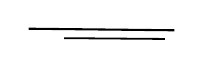
\begin{tikzpicture}[x=1cm,y=1cm]
\draw[line width=.75pt] (0,0) -- (1.85,-.02);
\draw[line width=.65pt] (.45,-.12) -- (1.73,-.13);
\end{tikzpicture}}

\deleted{$G$} $X$ affine scheme over $k$, \deleted{\unsure{of|and}} with $k$-algebra $\mathcal A$. We define $\check{\mathcal A}=\mathrm{Dist}(X\deleted{)},k)$. We \unsure{have|.} the functor $\inserted{k'}\rightarrow\mathrm{Dist}(X,k')$, denoted $\mathrm{Dis}(X)$, representable by $\mathbb V(A)$. We have
% slanted
\reversemarginpar\margin{\tikz[baseline=-.3ex,x=1em,y=1em]{\draw[->] (.56,.85) to[out=-130,in=76] (0,-.55);} \uline{covariant}}\normalmarginpar
\[
\left\{\begin{aligned}
&\text{a)}\ \mathrm{Dist}(X)\ \text{functorial in }X\quad
  (\text{as a Module over }\unsure{\mathcal O|O|\mathbb O}_k)\\
&\text{b)}\ \mathrm{Dist}(X)\times\mathrm{Dist}Y)
  \xrightarrow[\unsure{\pi|\Pi}_{X,Y}]{\deleted{\unsure{\alpha|o}}}
  \mathrm{Dist}(X\times Y)\quad\text{bilinear}
\end{aligned}\right.
\]
[and universal for bilinear homomorphisms from $\mathrm{Dis}(X)\times\mathrm{Dis}(Y)$ to a $\mathbb V(M)$] in fact inducing an isomorphism
\[
\mathrm{Dist}(X)\boxtimes\mathrm{Dist}(Y)\simeq\mathrm{Dist}(X\times Y).
\]

c) We have a functorial inclusion
\[
X\xrightarrow{\alpha_X}\mathrm{Dist}(X)
\]
[point distribution, compatible with passage to the product, i.e. we have commutativity of the
\diagram{\begin{tikzcd}[ampersand replacement=\&]
X\times Y \arrow[r,"\alpha_X\times\alpha_Y"] \arrow[dr,swap,"\unsure{\pi|\Pi}_{X\times Y}"] \& \unsure{\mathrm{Dist}}(X)\times\mathrm{Dist}(Y) \arrow[d,"\unsure{\pi|\Pi}_{X,Y}"]\\
\& \mathrm{Dist}(X\times Y)
\end{tikzcd}}

\deleted{If $G$ is equipped with a law of composition, $\mathrm{Dist}(G)$ too. \deleted{\unsure{If}} It is unital if and only if that of $\mathrm{Dist}(G)$ is} In fact we can reconstruct $X$ from $\mathrm{Dist}(X)=\mathbb D$ and the additional structure
\[
D\overset{\Delta}{\unsure{\mathbin{-}|\longrightarrow}}D\boxtimes D
\]
\margin{$[\,V(A)\boxtimes V(B)\overset{\text{def}}{\simeq}V(A\otimes B)\,]$\newline
[NB $\boxtimes=\otimes$ if $A$ or $B$ projective of finite type]}
% slanted
\reversemarginpar\margin{NB we reconstitute $X$ from $D$ equipped \deleted{\unsure{the|of the}}with the diagonal map $D\to D\boxtimes D$ commutative associative unital.}\normalmarginpar
must be an associative commutative and counital ``diagonal map'' [i.e. we have $D\xrightarrow{\varepsilon}\mathcal O$ \ldots.] as consisting of the \deleted{\unsure{points|gts}} $x\in\mathbb D(k')$ such that
\[
\boxed{\Delta(x)=x\boxtimes x}
\]
% archive sheet number: 21
